\documentclass[journal,12pt,twocolumn]{IEEEtran}

\usepackage{enumitem}
\usepackage{amsmath}
\usepackage{amssymb}
\usepackage{gensymb}
\usepackage{graphicx}
\usepackage{txfonts}         
\usepackage{listings}
\usepackage{lstautogobble}
\usepackage{mathtools}
\usepackage{bm}
\usepackage{hyperref}
\usepackage{polynom}
\usepackage{siunitx}
\usepackage{verbatim}
\usepackage[siunitx]{circuitikz}

\newcommand{\solution}{\noindent \textbf{Solution: }}
\providecommand{\pr}[1]{\ensuremath{\Pr\left(#1\right)}}
\providecommand{\brak}[1]{\ensuremath{\left(#1\right)}}
\providecommand{\cbrak}[1]{\ensuremath{\left\{#1\right\}}}
\providecommand{\sbrak}[1]{\ensuremath{\left[#1\right]}}
\providecommand{\mean}[1]{E\left[ #1 \right]}
\providecommand{\var}[1]{\mathrm{Var}\left[ #1 \right]}
\providecommand{\der}[1]{\mathrm{d} #1}
\providecommand{\gauss}[2]{\mathcal{N}\ensuremath{\left(#1,#2\right)}}
\providecommand{\mbf}{\mathbf}
\providecommand{\abs}[1]{\left\vert#1\right\vert}
\providecommand{\norm}[1]{\left\lVert#1\right\rVert}
\providecommand{\z}[1]{{\mathcal{Z}}\cbrak{#1}}
\providecommand{\ztrans}{\overset{\mathcal{Z}}{ \rightleftharpoons}}
\providecommand{\system}[1]{\overset{\mathcal{#1}}{ \longleftrightarrow}}
\providecommand{\parder}[2]{\frac{\partial}{\partial #2} \brak{#1}}

\let\StandardTheFigure\thefigure
\let\vec\mathbf

\numberwithin{equation}{section}
\numberwithin{figure}{section}
\renewcommand{\thefigure}{\theenumi}
\renewcommand\thesection{\arabic{section}}

\newcommand{\myvec}[1]{\ensuremath{\begin{pmatrix}#1\end{pmatrix}}}
\newcommand{\mymat}[1]{\ensuremath{\begin{bmatrix}#1\end{bmatrix}}}
\newcommand{\mydet}[1]{\ensuremath{\begin{vmatrix}#1\end{vmatrix}}}
\newcommand{\define}{\stackrel{\triangle}{=}}

\DeclareMathOperator*{\argmin}{arg\,min}
\DeclareMathOperator*{\argmax}{arg\,max}

\makeatletter
\def\pld@CF@loop#1+{%
    \ifx\relax#1\else
        \begingroup
          \pld@AccuSetX11%
          \def\pld@frac{{}{}}\let\pld@symbols\@empty\let\pld@vars\@empty
          \pld@false
          #1%
          \let\pld@temp\@empty
          \pld@AccuIfOne{}{\pld@AccuGet\pld@temp
                            \edef\pld@temp{\noexpand\pld@R\pld@temp}}%
           \pld@if \pld@Extend\pld@temp{\expandafter\pld@F\pld@frac}\fi
           \expandafter\pld@CF@loop@\pld@symbols\relax\@empty
           \expandafter\pld@CF@loop@\pld@vars\relax\@empty
           \ifx\@empty\pld@temp
               \def\pld@temp{\pld@R11}%
           \fi
          \global\let\@gtempa\pld@temp
        \endgroup
        \ifx\@empty\@gtempa\else
            \pld@ExtendPoly\pld@tempoly\@gtempa
        \fi
        \expandafter\pld@CF@loop
    \fi}
\def\pld@CMAddToTempoly{%
    \pld@AccuGet\pld@temp\edef\pld@temp{\noexpand\pld@R\pld@temp}%
    \pld@CondenseMonomials\pld@false\pld@symbols
    \ifx\pld@symbols\@empty \else
        \pld@ExtendPoly\pld@temp\pld@symbols
    \fi
    \ifx\pld@temp\@empty \else
        \pld@if
            \expandafter\pld@IfSum\expandafter{\pld@temp}%
                {\expandafter\def\expandafter\pld@temp\expandafter
                    {\expandafter\pld@F\expandafter{\pld@temp}{}}}%
                {}%
        \fi
        \pld@ExtendPoly\pld@tempoly\pld@temp
        \pld@Extend\pld@tempoly{\pld@monom}%
    \fi}
\makeatother

\lstset {
	frame=single, 
	breaklines=true,
	columns=fullflexible,
	autogobble=true
}             
                               
\title{Fourier Series \\ \Large EE3900- Linear Systems and Signal Processing \\ \large IIT Hyderabad}
\author{Adithya Ram Malothu \\ \normalsize BM20BTECH11009 \\ \vspace*{20pt} \normalsize 25th Oct 2022}

\begin{document}

	\maketitle

	\section{Periodic Function}
	Let 
	\begin{align}
		x(t) &= A_0\abs{\sin\brak{2\pi f_0 t}}
		\label{eq:10-orig-diff-def}
	\end{align}

	\begin{enumerate}[label=\thesection.\arabic*,ref=\thesection.\theenumi]
	\item Plot $x(t)$
	
	\solution Download the following Python code that plots Fig. \ref{fig-1.1}.
	\begin{lstlisting}
		wget https://github.com/adithyajadhav01/EE3900/blob/main/FOURIER/CODES/1.1.py
	\end{lstlisting}
	
	Run the code by executing
	\begin{lstlisting}
		python 1.1.py
	\end{lstlisting}

	\begin{figure}[!ht]
		\centering
		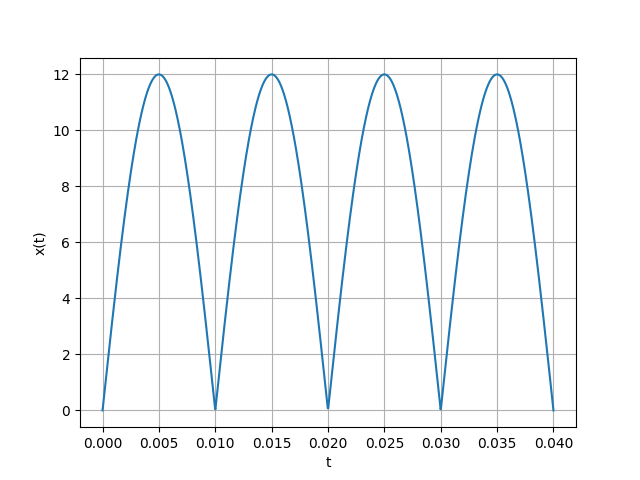
\includegraphics[width=\columnwidth]{./FIGURES/1.1.png}
		\caption{Plot of $x(t)$}
		\label{fig-1.1}	
	\end{figure}
	
	\item Show that $x(t)$ is periodic and find its period
	
	\solution Since $x(t)$ is the absolute value of a sinusoidal function, it is periodic, which is also evident from the plot
	
	Consider $x(t+\frac{1}{2f_0})$
	\begin{align}
		x\brak{t+\frac{1}{2f_0}} &= A_0 \abs{\sin\brak{2\pi f_0 \brak{t+\frac{1}{2f_0}}}} \\
		&= A_0 \abs{\sin\brak{2\pi f_0 t + \pi f_0}} \\
		&= A_0\abs{(-1)^{f_0} \sin\brak{2\pi f_0 t}} \\
		&= A_0\abs{\sin\brak{2\pi f_0 t}} \\
		&= x(t)
	\end{align}
	
	Therefore, $x(t)$ is periodic with period $\frac{1}{2f_0}$
	
	\end{enumerate}
	
	\section{Fourier Series}
	Consider $A_0 =12$ and $f_0 = 50$ for all numerical calculations
	\begin{enumerate}[label=\thesection.\arabic*,ref=\thesection.\theenumi]
	\item If
	\begin{align}
		x(t) = \sum_{k = -\infty}^{\infty}c_ke^{\j2\pi kf_0 t}
		\label{eq:one-Z-complex}
	\end{align}
	show that 
	\begin{align}
		c_k = f_0\int_{-\frac{1}{2f_0}}^{\frac{1}{2f_0}}x(t)e^{-\j2\pi kf_0 t}\, \der{t}
		\label{eq:one-Z}
	\end{align}
	
	\solution
	\begin{align}
    		x(t)e^{-\j2\pi nf_0t} &= \sum_{k = -\infty}^{\infty}c_ke^{-\j2\pi (n - k)f_0 t} \\
    		\implies \int_{-\frac{1}{2f_0}}^{\frac{1}{2f_0}} x(t)e^{-\j2\pi nf_0t} \,\der{t} &= \sum_{k = -\infty}^{\infty} c_k \int_{-\frac{1}{2f_0}}^{\frac{1}{2f_0}} e^{-\j2\pi (n - k)f_0 t} \,\der{t} 
	\end{align}
	
	But 
	\begin{align}
		\int_{-\frac{1}{2f_0}}^{\frac{1}{2f_0}} e^{-\j2\pi (n - k)f_0 t} \,\der{t} &=
		\begin{cases}
			\frac{1}{f_0} & k = n \\
			0 & k \ne n	
		\end{cases}	\\
		&= \frac{1}{f_0} \delta(n-k)
	\end{align}
	\begin{align}
		\sum_{k = -\infty}^{\infty} c_k \int_{-\frac{1}{2f_0}}^{\frac{1}{2f_0}} e^{-\j2\pi (n - k)f_0 t} \,\der{t} &= \sum_{k = -\infty}^{\infty} c_k \frac{1}{f_0} \delta(n-k) \\
		&= \frac{1}{f_0} c_n * \delta(n) \\
		&= \frac{1}{f_0} c_n
	\end{align}
	
	Therefore
	\begin{align}
		c_k = f_0\int_{-\frac{1}{2f_0}}^{\frac{1}{2f_0}}x(t)e^{-\j2\pi kf_0 t}\, \der{t}
	\end{align}
	
	\item Find $c_k$ for \eqref{eq:10-orig-diff-def}
	
	\solution
	\begin{align}
		c_k = f_0\int_{-\frac{1}{2f_0}}^{\frac{1}{2f_0}}A_0\abs{\sin\brak{2\pi f_0 t}}e^{-\j2\pi kf_0 t}\, \der{t}
	\end{align}
	\begin{multline}
		c_k = f_0\int_{-\frac{1}{2f_0}}^{0}A_0\brak{-\sin\brak{2\pi f_0 t}}e^{-\j2\pi kf_0 t}\, \der{t} \\ +f_0\int_{0}^{\frac{1}{2f_0}}A_0\brak{\sin\brak{2\pi f_0 t}}e^{-\j2\pi kf_0 t}\, \der{t}
	\end{multline}
	\begin{multline}
		c_k = f_0\int_{0}^{\frac{1}{2f_0}}A_0\sin\brak{2\pi f_0 u}e^{\j2\pi kf_0 u}\, \der{t} \\ +f_0\int_{0}^{\frac{1}{2f_0}}A_0\sin\brak{2\pi f_0 t}e^{-\j2\pi kf_0 t}\, \der{t}
	\end{multline}
	\begin{align}
		c_k &= f_0 \int_{0}^{\frac{1}{2f_0}} A_0\sin\brak{2\pi f_0 t} \brak{e^{\j2\pi kf_0 t} + e^{-\j2\pi kf_0 t}} \,\der{t} \\
		&= f_0A_0 \int_{0}^{\frac{1}{2f_0}} 2\sin\brak{2\pi f_0 t} \cos\brak{2\pi k f_0 t} \,\der{t} \\
		&= f_0A_0 \int_{0}^{\frac{1}{2f_0}} \cbrak{\sin\brak{2\pi(1+k)f_0t} + \sin\brak{2\pi(1-k)f_0t}} \,\der{t} \\
		&= f_0A_0 \sbrak{-\frac{\cos\brak{2\pi(1+k)f_0t}}{2\pi(1+k)f_0} - \frac{\cos\brak{2\pi(1-k)f_0t}}{2\pi(1-k)f_0}}_0^{\frac{1}{2f_0}} \\
		&= \frac{f_0A_0}{2\pi f_0} \sbrak{\frac{1-(-1)^{1+k}}{1+k} + \frac{1-(-1)^{1-k}}{1-k}} \\
		&= \brak{1 + (-1)^k} \frac{A_0}{2\pi} \sbrak{\frac{1}{1+k} + \frac{1}{1-k}} \\
		&= \brak{1 + (-1)^k} \frac{A_0}{\pi(1-k^2)}
	\end{align}
	
	Therefore
	\begin{align}
		c_k = 
		\begin{cases}
			\frac{2A_0}{\pi(1-k^2)} & k \text{ is even} \\
			0 & k \text{ is odd} 
		\end{cases}
	\end{align}
	
	\item Verify \eqref{eq:10-orig-diff-def} using Python
	
	\solution Download the following Python code that plots Fig. \ref{fig-2.3}.
	\begin{lstlisting}
		wget https://github.com/adithyajadhav01/EE3900/blob/main/FOURIER/CODES/2.3.py
	\end{lstlisting}
	
	Run the code by executing
	\begin{lstlisting}
		python 2.3.py
	\end{lstlisting}

	\begin{figure}[!ht]
		\centering
		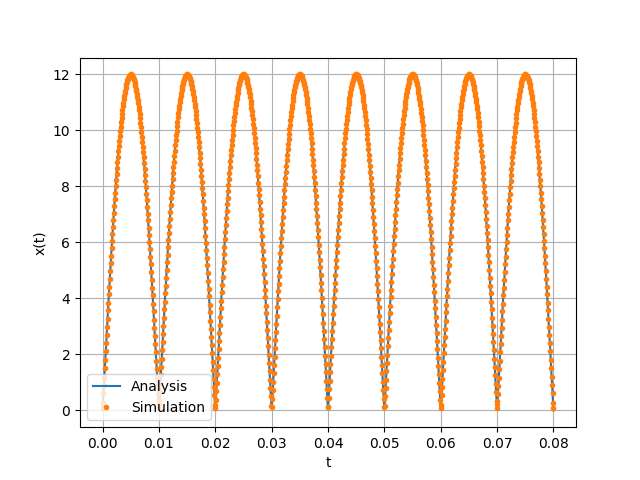
\includegraphics[width=\columnwidth]{./FIGURES/2.3.png}
		\caption{Plot of $x(t)$ along with its complex Fourier series expansion}
		\label{fig-2.3}	
	\end{figure}
	
	\item Show that 
	\begin{align}
		x(t) = \sum_{k = 0}^{\infty}\brak{a_k\cos{\brak{2\pi kf_0 t}}+b_k\sin{\brak{2\pi kf_0 t}}}
		\label{eq:one-Z-real}
	\end{align}
	and obtain the formulae for $a_k$ and $b_k$	
	
	\solution
	\begin{align}
    		x(t) &= \sum_{k = -\infty}^{\infty}c_ke^{\j2\pi kf_0 t} \\
        &= c_0 + \sum_{k = 1}^{\infty}c_ke^{\j2\pi kf_0t} + c_{-k}e^{-\j2\pi kf_0t} 
	\end{align}
	
	Thus
	\begin{multline}
		x(t) = c_0 + \sum_{k = 1}^{\infty}\brak{c_k + c_{-k}}\cos\brak{2\pi kf_0t}   \\
        + \sum_{k = 1}^{\infty}\j\brak{c_k - c_{-k}}\sin\brak{2\pi kf_0t}
	\end{multline}
	
	Therefore
	\begin{align}
    		a_k &= 
	    \begin{cases}
	        c_0 & k = 0 \\
    		    c_k + c_{-k} & k > 0
	    \end{cases} \\
    		b_k &= \j(c_k - c_{-k}) ~~ k \ge 0
	\end{align}	
	
	\item Find $a_k$ and $b_k$ for \eqref{eq:10-orig-diff-def}
	
	\solution 
	\begin{align}
		a_0 &= c_0 = \frac{2A_0}{\pi} 
	\end{align}
	
	For $k > 0$, if $k$ is odd
	\begin{align}
		a_k = 0 + 0 = 0
	\end{align}
	
	and if $k$ is even
	\begin{align}
		a_k = \frac{2A_0}{\pi(1-k^2)} + \frac{2A_0}{\pi(1-k^2)} = \frac{4A_0}{\pi(1-k^2)}
	\end{align}
	
	For odd or even $k$, $c_k = c_{-k}$ always
	\begin{align}
		b_k = 0 \quad \forall k \ge 0
	\end{align}
	
	Therefore
	\begin{align}
		a_k &=
		\begin{cases}
			\frac{2A_0}{\pi} & k = 0 \\
			\frac{4A_0}{\pi(1-k^2)} & k = 2m, m \in \mathbb{N} \\
			0 & \text{otherwise}
		\end{cases} \\
		b_k &= 0 \qquad \quad ~ k \ge 0
	\end{align}
	
	\item Verify \eqref{eq:one-Z-real} using Python
	
	\solution Download the following Python code that plots Fig. \ref{fig-2.6}.
	\begin{lstlisting}
		wget https://github.com/adithyajadhav01/EE3900/blob/main/FOURIER/CODES/2.6.py
	\end{lstlisting}
	
	Run the code by executing
	\begin{lstlisting}
		python 2.6.py
	\end{lstlisting}

	\begin{figure}[!ht]
		\centering
		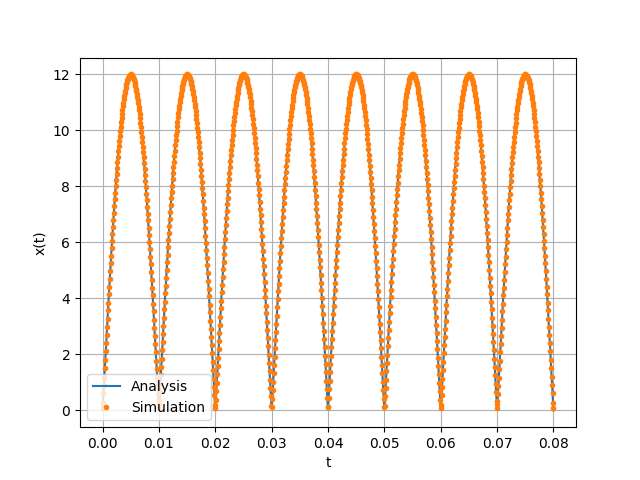
\includegraphics[width=\columnwidth]{./FIGURES/2.6.png}
		\caption{Plot of $x(t)$ along with its Fourier series expansion}
		\label{fig-2.6}	
	\end{figure}
	
	\begin{figure}[!ht]
		\centering
		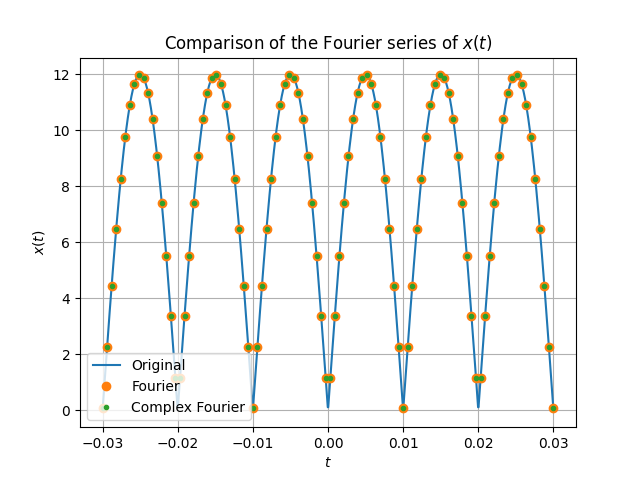
\includegraphics[width=\columnwidth]{./FIGURES/comparison.png}
		\caption{Comparison of the Fourier series of $x(t)$}
		\label{fig-comparison}	
	\end{figure}
	\end{enumerate}

	\section{Fourier Transform}
	\begin{enumerate}[label=\thesection.\arabic*,ref=\thesection.\theenumi]
	\item 
	\begin{align}
		\delta(t) &= 0 && t \ne 0 \\
		\int_{-\infty}^{\infty} \delta(t) &= 1
	\end{align}

	\item Find the Fourier transform of $x(t)$

	\solution 
	\begin{align}
		x(t) &= \sum_{k=-\infty}^\infty c_k e^{\j 2\pi kf_0t} \\
		\mathcal{F}\cbrak{x(t)} &= \sum_{k=-\infty}^\infty c_k \mathcal{F}\cbrak{e^{\j 2\pi kf_0t}}
	\end{align}
	\end{enumerate}
	\end{document}